% (The MIT License)
%
% Copyright (c) 2023-2024 Yegor Bugayenko
%
% Permission is hereby granted, free of charge, to any person obtaining a copy
% of this software and associated documentation files (the 'Software'), to deal
% in the Software without restriction, including without limitation the rights
% to use, copy, modify, merge, publish, distribute, sublicense, and/or sell
% copies of the Software, and to permit persons to whom the Software is
% furnished to do so, subject to the following conditions:
%
% The above copyright notice and this permission notice shall be included in all
% copies or substantial portions of the Software.
%
% THE SOFTWARE IS PROVIDED 'AS IS', WITHOUT WARRANTY OF ANY KIND, EXPRESS OR
% IMPLIED, INCLUDING BUT NOT LIMITED TO THE WARRANTIES OF MERCHANTABILITY,
% FITNESS FOR A PARTICULAR PURPOSE AND NONINFRINGEMENT. IN NO EVENT SHALL THE
% AUTHORS OR COPYRIGHT HOLDERS BE LIABLE FOR ANY CLAIM, DAMAGES OR OTHER
% LIABILITY, WHETHER IN AN ACTION OF CONTRACT, TORT OR OTHERWISE, ARISING FROM,
% OUT OF OR IN CONNECTION WITH THE SOFTWARE OR THE USE OR OTHER DEALINGS IN THE
% SOFTWARE.

\documentclass{article}
\usepackage{../osbp}
\newcommand*\thetitle{Integrating}
\begin{document}

\plush{\osbpTitlePage{6}{}}

\thought{Setup continuous integration in order to prove that your product works}

\qte
  [Pei Liu]
  {pei-liu}
  {We start by collecting a set of 84,475 open-source Android apps from the most popular three online code hosting sites, namely Github, GitLab, and Bitbucket. We then look into those apps and find that only around 10\% of apps have leveraged CI/CD services, i.e., the \ul{majority} of open-source Android apps are developed \ul{without} accessing CI/CD services.}
  {liu2022first}

\qte
  [Mehdi Golzadeh]
  {mehdi-golzadeh}
  {Together with Travis, GHA covers more than 80\% of all usages. Moreover, in only 18 months GHA has overtaken all other CIs in popularity.}
  {golzadeh2022rise}
\pitch{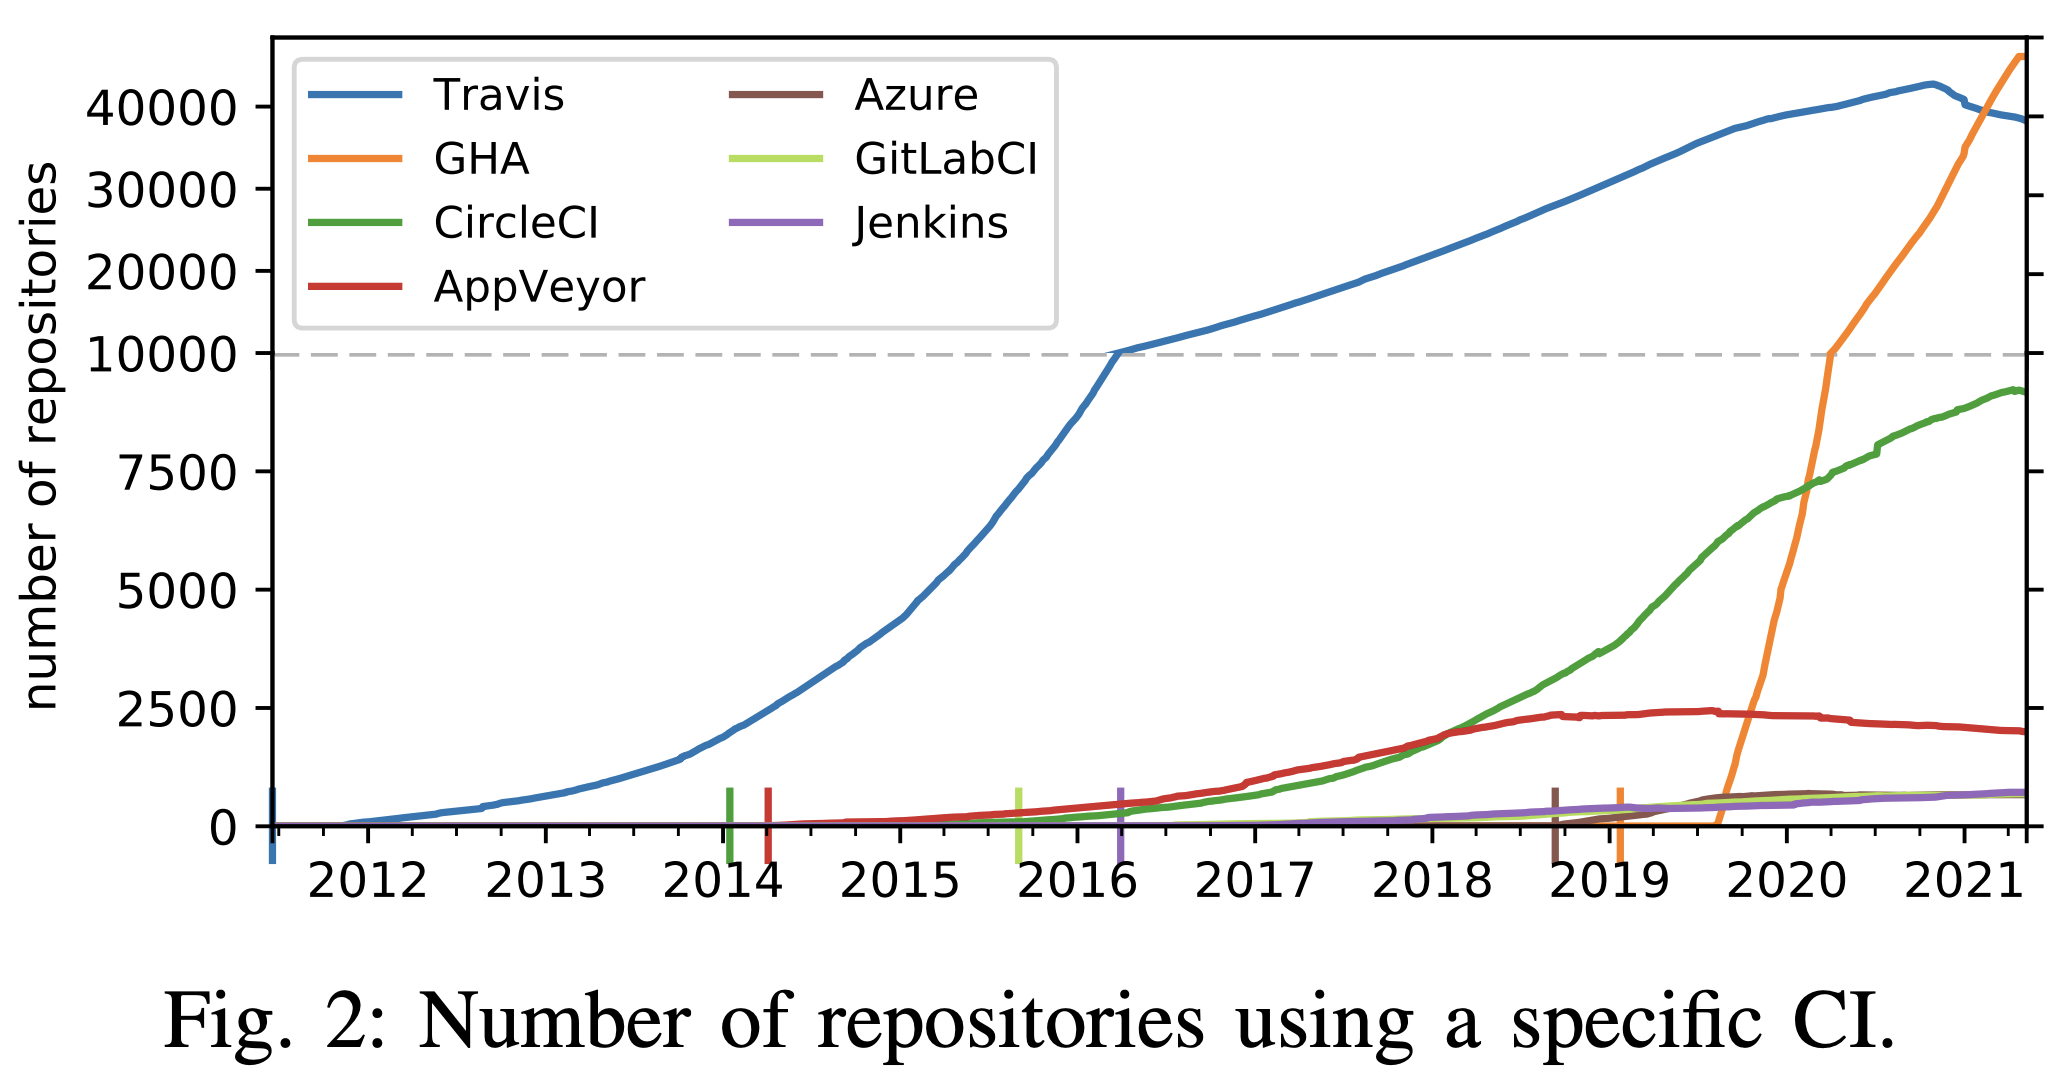
\includegraphics[width=.75\linewidth]{gha-growth.png}
  \source{golzadeh2022rise}}

\thought{Provide \ff{Dockerfile}}

\thought{Be aware of flaky tests}

\thought{Use fixed versions}

\thought{Enable renovate or dependabot}

\thought{Split tests on fast and slow}

\thought{Use caching in GitHub Action}

\thought{Implement your own GitHub Actions}

% G. Gousios, A. Zaidman, M.-A. Storey, and A. van Deursen, “Work Practices and Challenges in Pull-based Development: The Integrator’s Perspective,” in Proceedings of the 37th International Conference on Software Engineering (ICSE’15), 2015, pp. 358–368.
% Gousios et al. [18] determine that 75% of projects that use PRs also use CI.

\end{document}
